\documentclass[border=10pt]{standalone}
\usepackage{karnaugh-map}
\usepackage{tikz}

\begin{document}
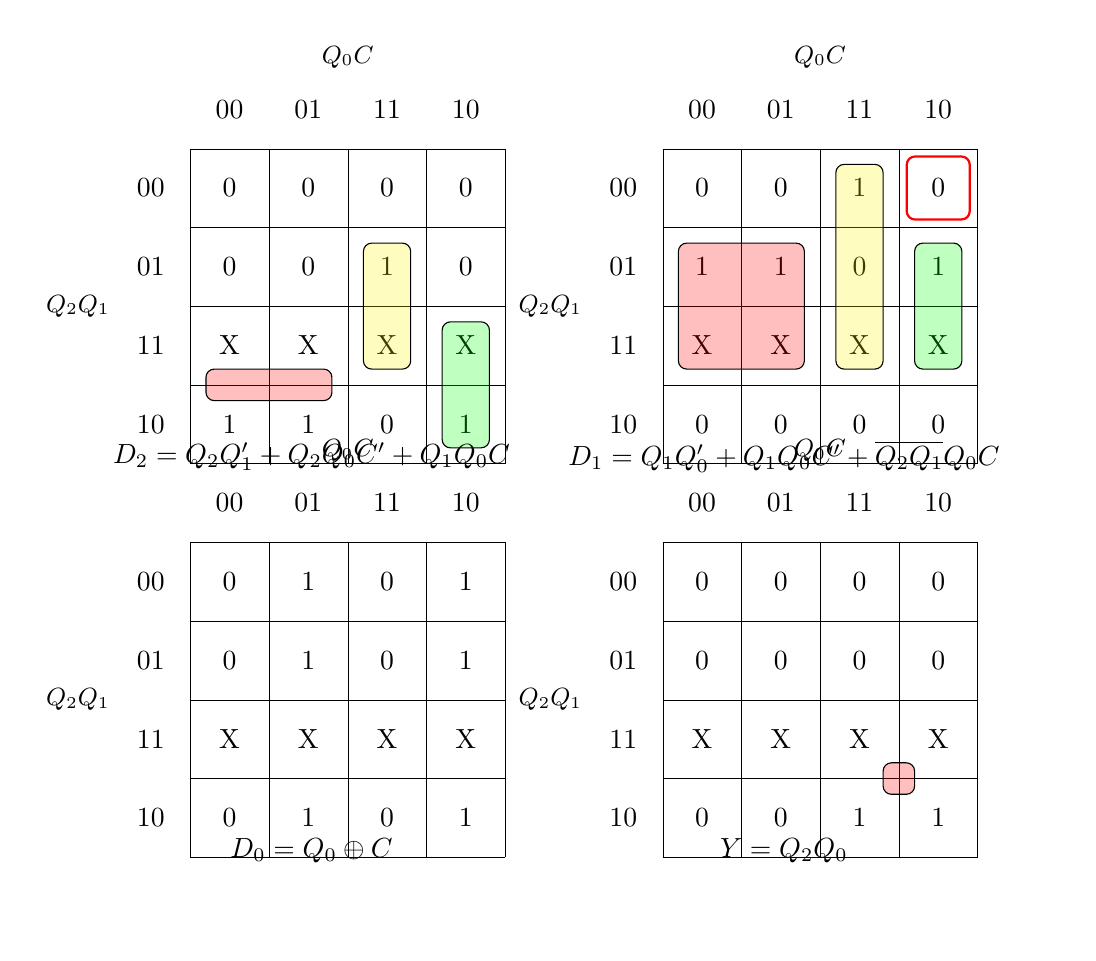
\begin{tikzpicture}
    % Variables: Rows Q2Q1, Cols Q0C
    % Order: Q2 Q1 Q0 C
    % Q2Q1: 00, 01, 11, 10
    % Q0C:  00, 01, 11, 10
    
    % D2 (Next Q2)
    % C=0: D2 = Q2
    % C=1: D2 = NextState (0->0, 1->0, 2->0, 3->1, 4->1, 5->0)
    % Minterms:
    % Q: 000 (0) -> C=0: 0, C=1: 0
    % Q: 001 (1) -> C=0: 0, C=1: 0
    % Q: 010 (2) -> C=0: 0, C=1: 0
    % Q: 011 (3) -> C=0: 0, C=1: 1 (00111=7)
    % Q: 100 (4) -> C=0: 1 (10000=16?), C=1: 1 (10001=17)
    % Q: 101 (5) -> C=0: 1 (10100=20), C=1: 0 (10101=21)
    % X: 110, 111 (24-27, 28-31)
    
    % Wait, mapping 4 variables: Q2, Q1, Q0, C.
    % Indices (binary Q2 Q1 Q0 C):
    % 0 (0000) -> 0
    % 1 (0001) -> 0
    % 2 (0010) -> 0
    % 3 (0011) -> 0
    % 4 (0100) -> 0
    % 5 (0101) -> 0
    % 6 (0110) -> 0
    % 7 (0111) -> 1 (State 3, C=1 -> Next 4 (100) -> D2=1)
    % 8 (1000) -> 1 (State 4, C=0 -> Hold 4 -> D2=1)
    % 9 (1001) -> 1 (State 4, C=1 -> Next 5 (101) -> D2=1)
    % 10 (1010) -> 1 (State 5, C=0 -> Hold 5 -> D2=1)
    % 11 (1011) -> 0 (State 5, C=1 -> Next 0 (000) -> D2=0)
    % 12-15 (11xx) -> X (Don't Care states 6,7)

    \node at (0, 5) {
        \begin{karnaugh-map}[4][4][1][$C$][$Q_0$][$Q_1$][$Q_2$]
            \minterms{7,8,9,10}
            \terms{12,13,14,15}{X}
            \autoterms[0]
            \implicant{8}{13} % Q2 Q1'
            \implicant{14}{10} % Q2 Q0 C'
            \implicant{7}{15}  % Q1 Q0 C
        \end{karnaugh-map}
    };
    \node at (0, 2.8) {$D_2 = Q_2 Q_1' + Q_2 Q_0 C' + Q_1 Q_0 C$};
    
    \node at (6, 5) {
        \begin{karnaugh-map}[4][4][1][$C$][$Q_0$][$Q_1$][$Q_2$]
            \minterms{3,4,5,6}
            \terms{12,13,14,15}{X}
            \autoterms[0]
            \implicant{4}{13} % Q1 Q0' (4,5,12,13)
            \implicant{6}{14} % Q1 Q0 C' (6,14)
            \implicant{3}{15} % Q1' Q0 C? (Check 3,15 match Q2' Q1' Q0 C in isolation, or Q0 C with X)
                              % 3 (0011), 7 (0111-0), 11 (1011-0), 15 (1111-X).
                              % Cannot simple group column.
                              % 3 (0011) adj 2 (0010-0), 1 (0001-0).
            % Actually, let's keep the explicit term Q2' Q1' Q0 C for 3.
            % Hard to show unconnected 1 on K-map clearly without visual group unless singular.
            \draw[rounded corners=3pt, fill=none, red, thick] (3.1, 3.1) rectangle (3.9, 3.9); % Highlight 3
        \end{karnaugh-map}
    };
    \node at (6, 2.8) {$D_1 = Q_1 Q_0' + Q_1 Q_0 C' + \overline{Q_2}\overline{Q_1}Q_0 C$};

    \node at (0, 0) {
        \begin{karnaugh-map}[4][4][1][$C$][$Q_0$][$Q_1$][$Q_2$]
            \minterms{1,2,5,6,9,10}
            \terms{12,13,14,15}{X}
            \autoterms[0]
        \end{karnaugh-map}
    };
    \node at (0, -2.2) {$D_0 = Q_0 \oplus C$};
    
    \node at (6, 0) {
        \begin{karnaugh-map}[4][4][1][$C$][$Q_0$][$Q_1$][$Q_2$]
            \minterms{10,11}
            \terms{12,13,14,15}{X}
            \autoterms[0]
            \implicant{10}{15} % Q2 Q0
        \end{karnaugh-map}
    };
    \node at (6, -2.2) {$Y = Q_2 Q_0$};

\end{tikzpicture}
\end{document}
